% Provenance (never printed): see sources/outline_sources.md (Year 2: oceanic islands; growth,
% flank collapse and erosion of volcanic islands; reefs and atolls; subsidence). Hawaiian
% stages, slides, subsidence and drowned reefs after Clague and Sherrod (2014, USGS PP 1801
% ch. 3) and Denlinger and Morgan (2014, ch. 4); the Nuuanu slide after the ODP Leg 200 report;
% the Enewetak holes after Ladd and Schlanger (1960, USGS PP 260-Y); Kure after the NOAA
% monument pages; the depth--age law from the Book 2 and Book 3 rows. Curves and the invented
% Petrel island from figdata/bachelor-2/islands.py; exercise and problem values in the Book 4
% scratch calculator calc/ch17.py.
\chapter{الجزر المحيطية}\label{ch:b2:oceanic-islands}

في عام 1952، على جزيرتين من حلقة إنيويتاك المرجانية في غرب المحيط الهادئ (وكان اسمها يُكتب
آنذاك إنيويتوك)، نزلت بئرا حفر عبر الصخر المرجاني إلى أكثر من \qty{1.2}{km}. وفي جزيرة باري
أخرج المثقب فتات بازلت طازج على عمق 4158 قدمًا، أي \qty{1267}{m}، ثم لبابًا من
بازلت أوليفيني. وفوقه حجر جيري من عمر الإيوسين، مليء بمرجانيات شعاب من نوع لا
ينمو أعمق من نحو \qty{46}{m}. فقد نمت شعاب مرجانية يومًا على كتفي بركان قرب مستوى
البحر، وغاص البركان أكثر من كيلومتر بينما ظلّت الشعاب تنمو فوقه. يتتبّع هذا
الفصل جزيرة محيطية طوال حياتها: كيف تنمو، وكيف تسقط أجنحتها في البحر، ولماذا
تغوص، وكيف يمكن لحلقة من المرجان أن تعيش بعدها.
% ledger: ls60:enewetak, ics4:eocene

\begin{recall}
\textbf{من مجلد السنة الأولى}: البقعة الساخنة، وعمود الوشاح، وأثر البقعة الساخنة وتدرّج أعماره،
وسلسلة هاواي--الإمبراطور وانتفاخ هاواي؛ وقانون العمق--العمر لقاع المحيط؛ والشعاب المرجانية،
وأنواعها الهدبية والحاجزية والحلقية كما وصفها داروين، وقاعدة «تابِع أو اغرق»؛
والسكونية ومستوى البحر في الذروة الجليدية الأخيرة، أخفض من اليوم بنحو \qty{120}{m}.
\textbf{من مجلدات المدرسة}: البركان الدرعي؛ ومصطبة نحت الأمواج.
\textbf{من \cref{ch:b2:magmatic-series}}: المتتاليتان الثولييتية والقلوية.
\end{recall}

\section{نموّ جزيرة بركانية}\label{sec:b2:oceanic-islands:growth}

جزر هاواي هي الطرف الأحدث من السلسلة التي تتبّعها مجلد السنة الأولى عبر شمال
المحيط الهادئ. وتضمّ الجزر الرئيسية 19 بركانًا درعيًا معروفًا: 15 منها فوق سطح البحر،
و3 مغمورة، وواحد، حديث الولادة، لا يزال تحت الماء. وبينما تحملها صفيحة المحيط الهادئ نحو
الشمال الغربي، يولد كلّ منها فوق البقعة الساخنة، وينمو، ثم يموت وهو ينجرف بعيدًا، ويغوص. وحياته
منتظمة بما يكفي لتُقسَم إلى مراحل.
% ledger: cs14:volcanoes

\begin{definition}[الجزيرة المحيطية؛ مراحل النموّ]\label{def:b2:oceanic-islands:stages}
\emph{الجزيرة المحيطية}\index{الجزيرة المحيطية} جزيرة بركانية ترتفع من قاع
المحيط، مبنيّة على غلاف صخري محيطي. وتمرّ جزيرة من سلسلة بقعة ساخنة بأربع مراحل
ثورانية: مرحلة \emph{ما قبل الدرع}، من ثورانات صغيرة لحمم قلوية على قاع البحر؛ ثم
\emph{مرحلة الدرع}\index{مرحلة الدرع}، التي تبني فيها الحمم الثولييتية معظم البركان
وهو فوق البقعة الساخنة؛ ثم مرحلة \emph{ما بعد الدرع}، من ثورانات أقلّ وأكثر قلوية،
تغطّي الدرع؛ ثم، بعد توقّف، مرحلة \emph{التجدّد}، من ثورانات قلوية نادرة
وصغيرة. ثم يتولّى الحتّ والغوص الأمر.
\end{definition}
% ledger: usgs14:hawaii-stages, cs14:rejuvenated

تتبع المراحل إمداد الحرارة. فلوئيهي، أحدث البراكين، يقع على بعد \qty{54}{km} جنوب
قمّة كيلاويا؛ ولا تزال قمّته تحت سطح البحر بمقدار \qty{975}{m}، لكنها ترتفع منذ الآن \qty{2.5}{km}
فوق قاع البحر من حوله، وأقدم حممه قلوية. وفي \omterm{def:b2:oceanic-islands:stages}{مرحلة الدرع} يقع البركان فوق
البقعة الساخنة ويُغذّى بأعلى معدّل. ويُقدَّر أن كل بركان في هاواي يُخرج من 80 إلى
\qty{95}{\percent} من حجمه النهائي في هذه المرحلة، ومعظمه في أول 1 إلى \qty{2}{Myr} من عمره.
وفي أواخر المرحلة ينخفض معدّل الثوران بعامل عشرة. فلا يعود ممكنًا إبقاء المستودعات الصهارية
الضحلة، على عمق 1 إلى \qty{7}{km}، حيّةً، وإن بقيت مستودعات أصغر على عمق 20 إلى \qty{30}{km}.
وتعود الحمم قلوية، لأن درجة انصهار أدنى تعطيها هذه الصفة، كما
بيّن \cref{ch:b2:magmatic-series}. وتأتي مرحلة التجدّد بعد توقّف يتراوح من أقلّ من 0.5
إلى \qty{2.0}{Myr}. وقد تكون نوبة أو نوبتين، أو طويلة جدًا: ففي نيئيهاو دامت من 2.2 إلى
\qty{0.4}{Ma}، وفي كاواي لا تزال مستمرة منذ \qty{3.5}{Ma}.
% ledger: cs14:loihi, usgs14:hawaii-stages, cs14:rejuvenated

الأحجام هائلة. فيُقدَّر حجم ماونا لوا بنحو \qty{74000}{km^3}. وحين يُعاد رسم الحدّ مع
كيلاويا بحيث لا يبقى لكيلاويا إلا نحو \qty{10000}{km^3}، ترتفع حصة ماونا لوا إلى
\qty{95600}{km^3}. ويحوي لوئيهي الفتيّ \qty{1700}{km^3}. وتبلغ السلسلة كلّها، منذ
\qty{81}{Ma}، نحو \qty{2e6}{km^3}؛ أمّا معدّل ثوران مُكامَل على ذلك التاريخ، \qty{0.07}{km^3}
في السنة، فيعطي قرابة ثلاثة أضعاف ذلك. والحمل ثقيل بما يكفي ليثني الصفيحة: فالقشرة
المحيطية تحت الجزر تنضغط نحو الأسفل بما يصل إلى \qty{5}{km}، على امتداد منخفض حلقي يُسمّى
منخفض هاواي الحلقي، ويرتفع انتفاخ منخفض، هو قوس هاواي، على بعد بضع مئات من الكيلومترات. أمّا
كيف تنثني صفيحة تحت حمل فيتناوله مجلد السنة الثالثة. والمنخفض الحلقي مهمّ هنا لأنه المكان الذي ينتهي إليه كثير من حطام الجزر.
% ledger: cs14:volumes, cs14:loihi, cs14:moat

\begin{omfigure}
\centering
\begin{tikzpicture}[x=0.95cm, y=0.95cm, font=\footnotesize]
% schematic, not to scale (vertical exaggeration about 10). Sea level y = 0; sea floor
% y = -1.6 - 0.0625 (16 - x), deepening with the age of the plate to the left.
\fill[omSea!45] (0,0) -- (16,0) -- (16,-1.6) -- (0,-2.6) -- cycle;
\fill[black!18] (0,-2.6) -- (16,-1.6) -- (16,-3.1) -- (0,-3.1) -- cycle;
\draw[black!60] (0,-2.6) -- (16,-1.6);
\draw[omSea!60!black] (0,0) -- (16,0);
\node[anchor=south, font=\scriptsize] at (8.7,0) {مستوى البحر};
% (a) shield stage over the hotspot
\fill[lith basalt, draw=black!70] (12.6,-1.8125) -- (13.9,0.75) -- (14.3,0.9) -- (14.7,0.75) -- (16,-1.6) -- cycle;
% (b) eroded island with a fringing reef (valleys notched in the summit)
\fill[lith basalt, draw=black!70] (9.2,-2.025) -- (10.1,0.15) -- (10.3,0.35) -- (10.45,0.2) -- (10.6,0.45) -- (10.8,0.25) -- (11.0,0.3) -- (11.2,0.1) -- (12.0,-1.85) -- cycle;
\fill[lith reef limestone, draw=black!70] (10.038,0) -- (9.976,-0.15) -- (9.80,0) -- cycle;
\fill[lith reef limestone, draw=black!70] (11.241,0) -- (11.303,-0.15) -- (11.46,0) -- cycle;
% (c) barrier reef around a smaller island, a lagoon between
\fill[lith basalt, draw=black!70] (5.8,-2.2375) -- (7.0,0.2) -- (8.2,-2.0875) -- cycle;
\fill[lith reef limestone, draw=black!70] (6.384,-1.05) -- (6.42,0) -- (6.60,0) -- (6.62,-0.45) -- (6.680,-0.45) -- cycle;
\fill[lith reef limestone, draw=black!70] (7.656,-1.05) -- (7.62,0) -- (7.44,0) -- (7.42,-0.45) -- (7.341,-0.45) -- cycle;
% (d) atoll: volcano bevelled and drowned, reef cap with a lagoon
\fill[lith basalt, draw=black!70] (2.7,-2.43125) -- (3.6,-0.55) -- (4.0,-0.55) -- (4.9,-2.29375) -- cycle;
\fill[lith reef limestone, draw=black!70] (3.4325,-0.9) -- (3.47,0) -- (4.14,0) -- (4.1806,-0.9) -- (4.0,-0.55) -- (3.6,-0.55) -- cycle;
\fill[omSea!45] (3.62,-0.15) rectangle (3.99,0);
% (e) guyot: flat top with a drowned reef cap, beyond the Darwin point
\fill[lith basalt, draw=black!70] (0.2,-2.5875) -- (0.9,-0.95) -- (1.7,-0.95) -- (2.4,-2.475) -- cycle;
\fill[lith reef limestone, draw=black!70] (0.9,-0.95) -- (0.96,-0.75) -- (1.64,-0.75) -- (1.7,-0.95) -- cycle;
% Darwin point
\draw[black!70, dashed] (2.55,0.55) -- (2.55,-2.5);
\node[anchor=south, font=\scriptsize] at (2.55,0.55) {نقطة داروين};
% hotspot and plate motion
\draw[omThm, line width=1.4pt, -{Stealth[length=2.5mm]}] (14.3,-3.9) -- (14.3,-3.15);
\node[anchor=west, font=\scriptsize, text=omThm] at (14.4,-3.7) {البقعة الساخنة};
\draw[black, line width=0.8pt, -{Stealth[length=2.5mm]}] (9.5,-2.85) -- (6.5,-2.85);
\node[anchor=west, font=\scriptsize] at (9.6,-2.85) {حركة الصفيحة};
\node[anchor=west, font=\scriptsize] at (0.1,-2.9) {الغلاف الصخري المحيطي};
% stage labels
\node[align=center, font=\scriptsize] at (14.3,1.45) {\foreignlanguage{arabic}{(أ) مرحلة الدرع}};
\node[align=center, font=\scriptsize] at (10.6,1.3) {\foreignlanguage{arabic}{(ب) جزيرة متآكلة،}\\ شعاب هدبية};
\node[align=center, font=\scriptsize] at (7.0,1.45) {\foreignlanguage{arabic}{(ج) شعاب حاجزية}};
\node[align=center, font=\scriptsize] at (3.8,1.45) {\foreignlanguage{arabic}{(د) حلقة مرجانية}};
\node[align=center, font=\scriptsize] at (1.3,1.45) {\foreignlanguage{arabic}{(ه) غيوت}};
\draw[black!60, -{Stealth[length=2mm]}] (13.6,-3.7) -- (0,-3.7);
\node[anchor=south, font=\scriptsize, fill=white, inner sep=1pt] at (7,-3.7) {براكين أقدم، وصفيحة أقدم وأعمق};
\end{tikzpicture}
\par\smallskip{\small حياة جزيرة محيطية، مقروءة على امتداد سلسلة بقعة ساخنة (تخطيطي، دون
مقياس رسم، والمقياس الرأسي مبالغ فيه كثيرًا). تحمل الصفيحة كلّ بركان بعيدًا عن البقعة الساخنة
(يمينًا) ويغوص البركان معها، بينما يبليه الحتّ. (أ)~بركان درعي ينمو فوق
البقعة الساخنة. (ب)~خامدًا ومتآكلًا، تحفّه الشعاب. (ج)~وقد غاص أكثر، تحيط به
شعاب حاجزية وخلفها بحيرة. (د)~غابت قمّته تحت البحر، وينمو فوقه غطاء من الشعاب
حول بحيرة وسطى، أي حلقة مرجانية. (ه)~وقد حُمل إلى ماء أبرد من أن تجاري فيه الشعاب
الغوص، تغرق \omterm{def:b2:oceanic-islands:reefs}{الحلقة المرجانية} وتغوص غيوتًا مسطّح القمّة.}
\end{omfigure}
% ledger: cs14:volcanoes, cs14:erase, cs14:darwin-point, pmnm:geology

\section{انهيار الجناح}\label{sec:b2:oceanic-islands:collapse}

ليس بركان يعلو عدّة كيلومترات، مبنيّ من مسيلات حمم مفكّكة وركام، قائم على منحدرات
تنزل إلى المنخفض الحلقي، بركانًا مستقرًا. ففي عام 1975 حرّك زلزال كالابانا، بقوّة 7.7،
الجناح الجنوبي لكيلاويا نحو البحر بما يصل إلى \qty{10}{m} دفعة واحدة وأثار تسونامي. وفي
عام 1868 رافقت حركة أخرى للجناح زلزالًا بقوّة 7.9 وتسونامي قتل 46
شخصًا. وتُظهر المقاطع الزلزالية تحت هذه الأجنحة عاكسًا عميقًا، يُقرأ على أنه
سطح انفصال على امتداد سطح القشرة المحيطية القديمة، ينزلق عليه الجناح كلّه. وعادةً
يزحف الجناح؛ وأحيانًا ينهار.
% ledger: dm14:flank

\begin{definition}[انهيار الجناح؛ الانهيار الركامي؛ الانزلاق الدوراني]\label{def:b2:oceanic-islands:collapse}
\emph{انهيار الجناح}\index{انهيار الجناح} هو انهيار جزء كبير من جناح
بركان، ينزلق بعيدًا تحت وزنه. وحين تتفتّت الكتلة المتحرّكة وتندفع
بسرعة، تيّارًا من الكتل والركام يمكن أن يقطع مسافات بعيدة وراء سفح البركان، فهو
\emph{انهيار ركامي}\index{الانهيار الركامي}. وحين تتحرّك ببطء، كتلًا كبيرة تدور
على صدوع متجذّرة في سطح انفصال عميق وتبقى قرب البركان، فهي \emph{انزلاق دوراني}.
\end{definition}

الدليل يرقد تحت البحر. ففي أواخر الثمانينيات، أظهرت خرائط السونار الجانبي للمياه المحيطة
بجزر هاواي حطامًا متناثرًا على قاع البحر العميق، على بعد عدّة مئات من الكيلومترات من
الجزر، وانزلاقات دورانية مكوّنة من كتل كبيرة مجزّأة. وقد تُعرّف على سبعة عشر انزلاقًا كبيرًا
حول الجزر الرئيسية، تكوّنت في آخر \qty{5}{Myr}. ويُعرف اليوم سبعون على امتداد
ظهرة هاواي بين جزيرة هاواي وميدواي، تكوّنت خلال \qty{30}{Myr}. أي انزلاق واحد على الأقلّ
كل \qty{300}{kyr} حول الجزر الرئيسية. وهذه الأعداد حدود دنيا، إذ يمكن لبركان
أحدث أن يدفن ندبة بركان أقدم وحطامه: فكالديرا القمّة ونطاق شقّ في
نيئيهاو مفقودان، ولم يُعثر لهما على أي رواسب. ويبدو أن الانزلاقات العملاقة أرجح حين
ينمو البركان بأسرع ما يكون، من أواخر مرحلة ما قبل الدرع إلى أوائل مرحلة ما بعد الدرع، لكنها تستمرّ
طويلًا بعد ذلك.
% ledger: cs14:slides, dm14:flank

أكبرها انزلاق نووانو، الذي اقتلع الجناح الشمالي الشرقي لبركان كوولاو
في أواهو. وهو \omterm{def:b2:oceanic-islands:collapse}{انهيار ركامي} منتشر على \qty{23000}{km^2}، يمتدّ أكثر من
\qty{200}{km} من الجزيرة. ومن كتله جبل توسكالوسا البحري، بطول نحو \qty{30}{km}،
وعرض \qty{17}{km} وارتفاع لا يقلّ عن \qty{2}{km}. وقد عبر الانهيار المنخفض الحلقي العميق وصعد
أكثر من \qty{100}{km} على منحدر قوس هاواي. ويُقدَّر عمره بين 2.1 و\qty{1.8}{Ma}،
قرب نهاية حياة كوولاو أو بعدها، وعمر حممه السطحية من 1.8 إلى
\qty{2.6}{Ma}. أمّا من كم انهيارًا تكوّن، وكم سمكه بعيدًا عن الجزيرة، فلا يزالان
سؤالين مفتوحين.
% ledger: odp200:nuuanu

\begin{omfigure}
\centering
\begin{tikzpicture}[x=0.95cm, y=0.95cm, font=\footnotesize]
% schematic section from the summit of an island (left) across the moat to the arch (right);
% not to scale. Sea level y = 0; top of the old oceanic crust, bent down under the island.
\fill[omSea!45] (0,0) -- (15,0) -- (15,-2.2) -- (13.5,-2.12) -- (11,-2.05) -- (8.5,-2.35) -- (6.5,-2.75) -- (5.6,-2.82) -- (4.0,-1.4) -- (2.5,0) -- cycle;
\fill[black!18] (0,-3.05) -- (5.6,-2.82) -- (6.5,-2.75) -- (8.5,-2.35) -- (11,-2.05) -- (13.5,-2.12) -- (15,-2.2) -- (15,-3.6) -- (0,-3.6) -- cycle;
\draw[black!70] (0,-3.05) -- (5.6,-2.82) -- (6.5,-2.75) -- (8.5,-2.35) -- (11,-2.05) -- (13.5,-2.12) -- (15,-2.2);
\draw[omSea!60!black] (0,0) -- (15,0);
\node[anchor=south east, font=\scriptsize] at (15,0) {مستوى البحر};
% the volcano: present flank (after collapse) and the lost flank (dashed)
\fill[lith basalt, draw=black!70] (0,1.15) -- (0.8,1.05) -- (1.25,0.95) -- (1.45,0.45) -- (1.75,0.1) -- (2.6,-0.75) -- (3.6,-1.6) -- (4.6,-2.4) -- (5.6,-2.82) -- (0,-3.05) -- cycle;
\draw[black!70, dashed] (1.25,0.95) -- (2.5,0) -- (4.0,-1.4) -- (5.6,-2.82);
\node[font=\scriptsize, align=center, fill=white, inner sep=1pt] at (0.8,-1.6) {البركان};
\node[font=\scriptsize, anchor=south west, align=left] at (2.0,0.25) {ندبة\\ الجناح المفقود};
% slump: blocks rotated on listric faults rooted in the decollement
\draw[black, line width=0.7pt] (1.45,0.45) .. controls (1.7,-1.4) and (2.4,-2.6) .. (3.6,-2.95);
\draw[black, line width=0.7pt] (2.6,-0.75) .. controls (2.8,-1.8) and (3.3,-2.6) .. (4.4,-2.9);
\draw[omThm, line width=1.1pt] (0.6,-3.03) -- (5.6,-2.82);
\node[anchor=north, font=\scriptsize, text=omThm] at (2.9,-3.05) {سطح الانفصال};
% debris avalanche: hummocky sheet across the moat and up the arch, with blocks
\fill[lith conglomerate, draw=black!70] (4.6,-2.4) -- (5.6,-2.62) -- (6.5,-2.6) -- (8.5,-2.22) -- (11,-1.95) -- (12.6,-2.03) -- (11,-2.05) -- (8.5,-2.35) -- (6.5,-2.75) -- (5.6,-2.82) -- cycle;
\fill[lith basalt, draw=black!70] (7.0,-2.62) -- (7.25,-2.25) -- (7.95,-2.22) -- (8.1,-2.43) -- cycle;
\fill[lith basalt, draw=black!70] (9.3,-2.2) -- (9.45,-2.02) -- (9.75,-2.0) -- (9.85,-2.17) -- cycle;
\fill[lith basalt, draw=black!70] (10.6,-2.05) -- (10.7,-1.93) -- (10.9,-1.92) -- (10.95,-2.03) -- cycle;
\draw[black!70] (7.6,-2.2) -- (7.4,-1.3) node[anchor=south, font=\scriptsize, align=center] {كتلة عرضها\\ عدّة كيلومترات};
\node[anchor=south, font=\scriptsize, align=center] at (10.3,-1.3) {انهيار ركامي};
\draw[black!70] (10.3,-1.3) -- (10.0,-1.98);
\node[font=\scriptsize] at (6.6,-3.2) {المنخفض الحلقي};
\node[font=\scriptsize] at (11.6,-2.6) {القوس};
\node[anchor=west, font=\scriptsize] at (12.6,-3.3) {قشرة محيطية};
\draw[black!70] (2.55,-1.55) -- (3.35,-0.6) node[anchor=west, font=\scriptsize, inner sep=1pt] {انزلاق دوراني};
\draw[black!60, {Stealth[length=2mm]}-{Stealth[length=2mm]}] (5.6,-3.95) -- (12.6,-3.95);
\node[anchor=north, font=\scriptsize] at (9.1,-3.95) {\foreignlanguage{arabic}{حتى نحو \mbox{\textdir TLT \qty{200}{km}}}};
\end{tikzpicture}
\par\smallskip{\small انهيار جناح جزيرة محيطية (تخطيطي، دون مقياس رسم). قرب
البركان يتحرّك انزلاق دوراني ببطء، كتلًا تدور على صدوع متجذّرة في سطح انفصال عند سطح
القشرة المحيطية القديمة. وينفصل \omterm{def:b2:oceanic-islands:collapse}{انهيار ركامي} عن الجناح، تاركًا ندبة، ويندفع
صفيحةً من الركام تحمل كتلًا عرضها عدّة كيلومترات. وقد عبر انهيار نووانو المنخفض الحلقي
وصعد على القوس، على بعد أكثر من \qty{200}{km} من أواهو.}
\end{omfigure}
% ledger: dm14:flank, odp200:nuuanu, cs14:moat

الانزلاق الذي يسقط في البحر يزيح الماء. ففي لاناي ومولوكاي تعلو بريشيات فوضوية
من المرجان والحمم حتى \qty{155}{m} فوق مستوى البحر، وقد قُرئت على أنها رواسب
أمواج عملاقة أثارتها الانهيارات. وهذه القراءة موضع جدل. فبعض المؤلفين يفسّرون الرواسب
بارتفاع الجزر، مع أن الشعاب الغارقة جنوب لاناي لا تُظهر أي أثر لارتفاع كهذا.
ونحو ثلث الانزلاقات العملاقة في هاواي كانت انهيارات ركامية قادرة على إثارة أمواج هائلة. أمّا كيف
يُوزن خطر كهذا، نادر لكنه كبير جدًا، فسؤال يعود إلى \cref{ch:b2:geological-hazards}.
% ledger: cs14:megatsunami

\section{لماذا تغوص الجزر المحيطية}\label{sec:b2:oceanic-islands:subsidence}

عمليّتان تجعلان \omterm{def:b2:oceanic-islands:stages}{الجزيرة المحيطية} تغوص، وتتداخلان. الأولى التحميل: فمع نموّ البركان
يدفع وزنه الصفيحة نحو الأسفل. وتدوم هذه المرحلة السريعة نحو مليون سنة ربما، وتُغرق
الشواطئ والشعاب بأكثر من كيلومتر. وقبالة الساحل الشمالي الغربي لجزيرة هاواي تعطي
شعاب غارقة مؤرَّخة معدّل غوص قدره \qty{2.6}{m} لكل ألف سنة. ويمكن لبركان صغير أن
يغرق كلّه في هذه المرحلة: فماهوكونا، بجوار جزيرة هاواي، كان جزيرة لفترة وجيزة، وقمّته
اليوم على عمق نحو \qty{1100}{m} تحت الماء.
والعملية الثانية هي تبرّد الصفيحة، الذي
يستمرّ مئة مليون سنة، والذي يضعه هذا القسم في أرقام.
% ledger: cs14:subsidence, cs14:mahukona

قاس مجلد السنة الأولى كيف يتعمّق قاع المحيط مع عمره $t$ (بوحدة \unit{Myr}). وبالصيغة
المستعملة في هذا الفصل:
\[
d(t) = \qty{2500}{m} + C\sqrt{t}, \qquad C = \qty{350}{m.Myr^{-1/2}}, \qquad 0 \le t \le 70,
\]
ومن أجل الصفائح التي يزيد عمرها على نحو \qty{20}{Myr}،
\[
d(t) = \qty{6400}{m} - \qty{3200}{m}\; e^{-t/62.8}.
\]
تتّفق الصيغتان في حدود نحو \qty{20}{m} بين 20 و\qty{50}{Myr}، وتتقاطعان عند
\qty{26}{Myr}.
% ledger: ps77:depth-age (Book 2), parsons:plate-model (Book 3)
% values (islands.py): t_switch 26.27, d_switch 4293.8; root - exp: 20 Myr -7.6, 50 Myr +18.3

\begin{proposition}[الغوص الحراري لجزيرة]\label{prop:b2:oceanic-islands:sinking}
جزيرة مبنيّة على صفيحة عمرها $t_1$، محمولة مع الصفيحة، تحمّلها بوزن
لم يعد يتغيّر ولا تغيّر تبرّد الصفيحة تحتها، تغوص بمقدار
\[
S = d(t_2) - d(t_1)
\]
حين تبلغ الصفيحة العمر $t_2$، بالمعدّل $\dot S = d'(t)$. ومع قانون الجذر،
\[
S = C\left(\sqrt{t_2} - \sqrt{t_1}\right), \qquad \dot S = \frac{C}{2\sqrt t},
\]
ومع القانون الأسّي، $\dot S = (\qty{3200}{m}/\qty{62.8}{Myr})\,e^{-t/62.8}$. وعلى فترة
معلومة، تحمل صفيحة فتيّة جزرها إلى أعمق مما تحملها صفيحة قديمة.
\end{proposition}

\begin{proof}
قارن بين عمودين من الصفيحة، لهما العمر نفسه، أحدهما تحت الجزيرة والآخر تحت المحيط
المفتوح بعيدًا. كلاهما يبرد بالطريقة نفسها، لأن الجزيرة لا تغيّر تبرّد الصفيحة. فكلاهما ينكمش بالمقدار نفسه، وينزل سطح كلّ منهما بالمقدار
نفسه. ووزن الجزيرة نفسه متوازن منذ قبل ولم يعد يتغيّر، فلا يضيف شيئًا
آخر. وينزل عمود المحيط المفتوح بمقدار $d(t_2) - d(t_1)$؛ وكذلك الجزيرة. وبالاشتقاق
نحصل على المعدّل. أمّا الادّعاء الأخير: فعلى فترة ثابتة $\Delta$، يتناقص $C(\sqrt{t_1 + \Delta} -
\sqrt{t_1})$ كلّما كبر $t_1$، لأن مشتقّه، $\frac C2\bigl(1/\sqrt{t_1 + \Delta}
- 1/\sqrt{t_1}\bigr)$، سالب.
\end{proof}

تُغفل القضيّة أمرين عن قصد. فانتفاخ البقعة الساخنة يرفع الصفيحة وهي تمرّ
ثم يُنزلها وهي تبتعد، وهذا يضاف إلى غوص أحدث الجزر
(وقد قاس مجلد السنة الأولى الانتفاخ). والحمل يتغيّر بينما ينمو البركان، وتلك هي
المرحلة السريعة أعلاه. فإذا انقضى كلاهما، تبعت الجزيرة القاع.

المعدّلات صغيرة. فعلى صفيحة عمرها \qty{4}{Myr} يعطي قانون الجذر \qty{87.5}{m} لكل مليون
سنة، أي أقلّ من عُشر مليمتر في السنة. وعلى صفيحة عمرها \qty{100}{Myr} يعطي القانون الأسّي
\qty{10.4}{m} لكل مليون سنة، أي \qty{0.01}{m} لكل ألف سنة. وهذا هو المعدّل
المقيس على امتداد معظم ظهرة هاواي وجبال الإمبراطور البحرية. أمّا مرحلة التحميل، بمعدّل
\qty{2.6}{m} لكل ألف سنة، فأسرع بنحو 250 مرة.
% ledger: cs14:subsidence; values (islands.py): rate_100 10.37, age_rate10 102.3

\begin{omfigure}
\centering
% figdata/bachelor-2/islands.py part sink
\begin{tikzpicture}
\begin{axis}[width=0.8\linewidth, height=6.2cm, y dir=reverse, xmin=0, xmax=100, ymin=0,
  ymax=3000, xlabel={الزمن منذ بناء الجزيرة \babelsublr{(\unit{Myr})}},
  ylabel={الغوص الحراري \babelsublr{(\unit{m})}}, tick label style={font=\scriptsize},
  label style={font=\small}, xtick pos=bottom, ytick pos=left]
\addplot[omThm, line width=1pt] table[x=dt_Myr, y=t2] {figdata/out/bachelor-2-islands-sink.dat};
\addplot[orange!80!black, line width=1pt] table[x=dt_Myr, y=t10] {figdata/out/bachelor-2-islands-sink.dat};
\addplot[blue!70!black, line width=1pt] table[x=dt_Myr, y=t30] {figdata/out/bachelor-2-islands-sink.dat};
\addplot[black!45, line width=1pt] table[x=dt_Myr, y=t60] {figdata/out/bachelor-2-islands-sink.dat};
\node[font=\scriptsize, anchor=south east, inner sep=1pt] at (axis cs:99,2470) {\foreignlanguage{arabic}{صفيحة عمرها \mbox{\textdir TLT \qty{2}{Myr}}}};
\node[font=\scriptsize, anchor=south east, inner sep=1pt] at (axis cs:99,2140) {\mbox{\textdir TLT \qty{10}{Myr}}};
\node[font=\scriptsize, anchor=south east, inner sep=1pt] at (axis cs:99,1380) {\mbox{\textdir TLT \qty{30}{Myr}}};
\node[font=\scriptsize, anchor=south east, inner sep=1pt] at (axis cs:99,710) {\mbox{\textdir TLT \qty{60}{Myr}}};
\draw[black!50, dashed] (axis cs:0,1267) -- (axis cs:58,1267);
\node[font=\scriptsize, anchor=north west, inner sep=1pt] at (axis cs:1,1300) {\foreignlanguage{arabic}{إنيويتاك، \mbox{\textdir TLT \qty{1267}{m}}}};
\end{axis}
\end{tikzpicture}
\par\smallskip{\small الغوص الحراري لجزيرة تحملها صفيحتها، من قانون العمق--العمر،
لجزر مبنيّة على صفائح أعمارها 2 و10 و30 و\qty{60}{Myr} (قانون الجذر حتى عمر للصفيحة قدره
\qty{26}{Myr}، والقانون الأسّي بعده، حيث يلتقيان). وكلّما كانت الصفيحة أفتى، غاصت الجزيرة أسرع
وأعمق. ويُعلّم الخطّ المتقطّع عمق البازلت تحت إنيويتاك، أي سمك
الصخر الشعابي الذي على الغوص أن يفسح له المكان.}
\end{omfigure}
% ledger: ps77:depth-age (Book 2), parsons:plate-model (Book 3), ls60:enewetak

\section{الشعاب والحلقات المرجانية والغيوتات}\label{sec:b2:oceanic-islands:reefs}

وصف مجلد السنة الأولى أنواع الشعاب الثلاثة كما فسّرها داروين، من شعاب تحفّ
جزيرة إلى حلقة من المرجان حول بحيرة، وانتهى بسؤال: لماذا تغوص الجزر،
وإلى أيّ حدّ؟ وقد أجاب القسم السابق عنه. فيمكن الآن تعريف الأنواع بحالة
الجزيرة تحتها.

\begin{definition}[الشعاب الهدبية؛ الشعاب الحاجزية؛ الحلقة المرجانية]\label{def:b2:oceanic-islands:reefs}
\emph{الشعاب الهدبية}\index{الشعاب الهدبية} شعاب متّصلة بشاطئ جزيرة، ليس بينهما
بحيرة، أو ليس بينهما إلا قناة ضيّقة ضحلة. و\emph{الشعاب الحاجزية}\index{الشعاب الحاجزية}
شعاب يفصلها عن الشاطئ بحيرة، على أجنحة جزيرة غاصت بينما
نمت الشعاب نحو الأعلى. و\emph{الحلقة المرجانية}\index{الحلقة المرجانية} حلقة من الشعاب، عليها جزر منخفضة من حطام الشعاب،
حول بحيرة ليس فوق مستوى البحر فيها أي صخر بركاني: فبركانها يقع كلّه تحت الشعاب.
\end{definition}

\begin{definition}[الجبل البحري؛ الغيوت]\label{def:b2:oceanic-islands:seamount}
\emph{الجبل البحري}\index{الجبل البحري} بركان على قاع المحيط تقع قمّته تحت مستوى
البحر، إمّا لأنه لم يبلغ السطح قط وإمّا لأنه غاص. و\emph{الغيوت}\index{الغيوت}
جبل بحري مسطّح القمّة، سطّحته الأمواج أو غطّته الشعاب حين
كان عند مستوى البحر، ثم غرق.
\end{definition}

إذا أبقت الشعاب قمّتها عند مستوى البحر بينما يغوص البركان تحتها، تراكم الصخر الشعابي بالسرعة
نفسها التي تنزل بها الجزيرة. فيسجّل سمك الغطاء عندئذٍ الغوص.

\begin{proposition}[سمك غطاء الشعاب]\label{prop:b2:oceanic-islands:cap}
لينزل آخر صخر بركاني لجزيرة تحت مستوى البحر حين يكون عمر صفيحتها $t_1$، ولتُبقِ
شعاب قمّتها عند مستوى البحر منذ ذلك الحين، حتى يصير عمر الصفيحة $t_2$. فإذا ارتفع مستوى البحر
بمقدار $\Delta\eta$ بين الزمنين (بالنسبة إلى مركز الأرض)، كان سمك غطاء الشعاب
فوق البركان
\[
H = d(t_2) - d(t_1) + \Delta\eta = C\left(\sqrt{t_2} - \sqrt{t_1}\right) + \Delta\eta
\]
والصيغة الثانية بقانون الجذر. ولا يتوقّف على المعدّل الذي يمكن أن تنمو به الشعاب،
شرط ألّا يكون ذلك المعدّل أصغر قط من الارتفاع النسبي لمستوى البحر.
\end{proposition}

\begin{proof}
عند $t_1$ تكون قمّة البركان عند مستوى البحر؛ وعند $t_2$ تقع أخفض بمقدار $S = d(t_2) - d(t_1)$ بحسب
\cref{prop:b2:oceanic-islands:sinking}، بينما ارتفع سطح البحر بمقدار $\Delta\eta$. وقمّة
الشعاب عند سطح البحر في الزمنين، وقاعدتها قمّة البركان. فالسمك
هو المسافة بينهما، $S + \Delta\eta$. والشعاب التي تجاري تتوقّف عند
السطح، فالشعاب الأسرع لا تبني غطاءً أسمك؛ والشعاب التي لا تستطيع المجاراة تتخلّف
وتغرق، وهي القاعدة المستعادة من مجلد السنة الأولى.
\end{proof}

تؤكّد إنيويتاك ذلك. فبقانون الجذر، يحتاج غطاء سمكه \qty{1267}{m} إلى $\sqrt{t_2} - \sqrt{t_1} =
1267/350 = 3.62$: مثلًا، بركان سُطّح حتى مستوى البحر على صفيحة عمرها \qty{10}{Myr}
وحُمل حتى صار عمر الصفيحة \qty{46}{Myr}. أي \qty{36}{Myr}، وهي رتبة الزمن الذي
يفصل قاعدة الحجر الجيري الإيوسينية عن اليوم. وقد أظهرت آبار الحفر أيضًا ما
تُغفله القضيّة. فالنطاقات المغسولة، حيث ذاب أراغونيت المرجانيات أو
أعيد تبلوره، تسجّل أزمنة كانت فيها قمّة \omterm{def:b2:oceanic-islands:reefs}{الحلقة المرجانية} فوق البحر ويهطل عليها المطر.
فمستوى البحر ينخفض ويرتفع مع العصور الجليدية، وقد انكشف الغطاء ثم غرق من جديد مرّات
كثيرة في طريقه نحو الأسفل.
% ledger: ls60:enewetak, ics4:eocene; calc/ch17.py: (3.162 + 3.620)^2 = 46.0

\begin{history}[الحفر عبر الحلقات المرجانية، 1896--1952]
قدّمت نظرية داروين تنبّؤًا لا يمكن التحقّق منه إلا بمثقب: فتحت \omterm{def:b2:oceanic-islands:reefs}{الحلقة المرجانية} ينبغي
أن تكون كومة سميكة من صخر شعابي من المياه الضحلة، مستقرّة على صخر بركاني. وأوّل بئر عميقة
على حلقة مرجانية في المحيط الهادئ حُفرت في فونافوتي من 1896 إلى 1898 وتوقّفت عند 1114 قدمًا،
أي \qty{340}{m}، دون أن تبلغ البركان. وبلغت بئر في كيتا دايتو جيما، جنوب اليابان وشرق أوكيناوا،
1416 قدمًا عام 1936، وبلغت بئر في بيكيني 2556 قدمًا عام 1947، ولم تبلغه أيّ منهما. وكانت آبار إنيويتاك، في
1951 و1952، أولى الآبار التي بلغت أساس حلقة مرجانية. ففي إلوغيلاب صودف الأساس الصلب
عند 4610 أقدام؛ وفي جزيرة باري البازلت عند 4158 قدمًا، أي أعلى بمقدار 450 قدمًا، على بعد \num{22}~ميلًا.
فقد وجد الحفّارون بركانًا بازلتيًا يرتفع ميلين فوق قاع المحيط، يغطّيه
حجر جيري شعابي منذ الإيوسين. ودُمّرت إلوغيلاب في تجربة لجهاز نووي حراري
بعد انتهاء الحفر بوقت قصير.
\end{history}
% ledger: ls60:holes, ls60:enewetak

\begin{omfigure}
\centering
% figdata/bachelor-2/islands.py part holes
\begin{tikzpicture}
\begin{axis}[width=0.8\linewidth, height=6.0cm, ybar, bar width=16pt, y dir=reverse, ymin=0,
  ymax=1500, enlarge x limits=0.1, symbolic x coords={Funafuti,Kita-daito-jima,Bikini,Eniwetok-K-1B,Eniwetok-F-1,Eniwetok-E-1},
  xtick=data, xticklabels={{فونافوتي\\1898},{كيتا دايتو جيما\\1936},{بيكيني\\1947},{إنيويتاك\\\mbox{\textdir TLT K-1B, 1951}},{إنيويتاك\\\mbox{\textdir TLT F-1, 1952}},{إنيويتاك\\\mbox{\textdir TLT E-1, 1952}}},
  xticklabel style={align=center, font=\scriptsize}, ylabel={العمق \babelsublr{(\unit{m})}},
  tick label style={font=\scriptsize}, label style={font=\small}, xtick pos=bottom, ytick pos=left]
\addplot[fill=omLithLime, draw=black!70] table[x=name, y=td_m] {figdata/out/bachelor-2-islands-holes.dat};
\addplot[only marks, mark=-, mark size=9pt, line width=2.2pt, black, unbounded coords=discard, xshift=0pt]
  table[x=name, y=basalt_m] {figdata/out/bachelor-2-islands-holes.dat};
\end{axis}
\end{tikzpicture}
\par\smallskip{\small الآبار العميقة المحفورة في حلقات مرجانية بالمحيط الهادئ، مع سنة إتمام كلّ منها:
عمقها الكلّي (الأعمدة)، وفي إنيويتاك عمق القاعدة البازلتية (العلامات السوداء)
(تحت إلوغيلاب في البئر \babelsublr{F-1} على عمق \qty{1405}{m}، وتحت جزيرة باري في البئر \babelsublr{E-1} على عمق \qty{1267}{m} من السطح). والأعماق محوّلة
من أقدام تقرير الحفر.}
\end{omfigure}
% ledger: ls60:holes, ls60:enewetak; values (islands.py): td and basalt in m

\begin{inthefield}[حفر حلقة مرجانية]
في إنيويتاك وضع الجيولوجيون الآبار العميقة قرب شاطئ البحيرة، حيث توقّعوا
كهوفًا أقلّ مما قرب الحافة البحرية للشعاب. وحُفر معظم البئر حفرًا مباشرًا، والصخر يُطحن إلى
فتات يرفعه سائل الحفر. وكان الفتات يصل متأخّرًا، فقدّر الفريق هذا
التأخّر ليعرف من أيّ عمق جاءت كل عيّنة. وعند أعماق مختارة أخذت أسطوانة اللباب أسطوانة
صلبة من الصخر. ولمّا انتهى الحفر، استُعملت الآبار أدوات قياس. ففي إحداها، المبطّنة
تبطينًا مصمتًا حتى \qty{600}{m}، ظلّ مستوى الماء يرتفع وينخفض مع مدّ المحيط وجزره، متزامنًا معه
وبالمقدار نفسه: فالحجر الجيري للغطاء مسامي ومليء بالكهوف في كلّ أجزائه. وفي آبار أخرى
قيست الحرارة وهي تعود إلى التوازن.
\end{inthefield}
% ledger: ls60:methods, ls60:casing (F-1 cased to 1,973 ft = 601 m)

لا يُحكم على الشعاب بالغرق لأن جزيرتها تغوص. فالمرجانيات والطحالب المرجانية تبني
مليمترات في السنة: ففي دراسة حديثة، نمت شعاب تسودها المرجانيات المتفرّعة \qty{4.2}{mm} في
السنة. أمّا
الصفيحة المتبرّدة فلا تأخذ إلا عُشر مليمتر في السنة على الأكثر. ولن يسبق الغوص الحراري وحده
شعابًا سليمة أبدًا. فالشعاب تغرق حين يتغيّر شيء آخر: حين تحملها الصفيحة إلى ماء
أبرد من أن يسمح بنموّ سريع؛ أو حين يرتفع مستوى البحر أسرع مما تستطيع مجاراته؛ أو حين يحدث الأمران معًا.
% ledger: perry:chagos (Book 3), cs14:darwin-point

\begin{omfigure}
\centering
% figdata/bachelor-2/islands.py part rates; horizontal lines from the ledger rows
\begin{tikzpicture}
\begin{semilogyaxis}[width=0.8\linewidth, height=6.4cm, xmin=0, xmax=150, ymin=0.005, ymax=100,
  xlabel={عمر الصفيحة \babelsublr{(\unit{Myr})}}, ylabel={المعدّل \babelsublr{(\unit{mm.yr^{-1}})}},
  tick label style={font=\scriptsize}, label style={font=\small}, xtick pos=bottom, ytick pos=left]
\addplot[omThm, line width=1.1pt] table[x=t_Myr, y=thermal_mm_yr] {figdata/out/bachelor-2-islands-rates.dat};
\draw[omThm, densely dotted, line width=0.9pt] (axis cs:75,0.01) -- (axis cs:150,0.01);
\node[font=\scriptsize, anchor=south west, inner sep=1pt, text=omThm] at (axis cs:22,0.042) {الغوص الحراري للصفيحة};
\node[font=\scriptsize, anchor=south west, inner sep=1pt, text=omThm] at (axis cs:96,0.0108) {مقيس، ظهرة هاواي};
\draw[black!70, line width=0.9pt] (axis cs:0,2.6) -- (axis cs:150,2.6);
\node[font=\scriptsize, anchor=north west, inner sep=1pt] at (axis cs:2,2.6) {التحميل، قبالة جزيرة هاواي};
\draw[green!50!black, line width=0.9pt] (axis cs:0,4.2) -- (axis cs:150,4.2);
\node[font=\scriptsize, anchor=south west, inner sep=1pt, text=green!40!black] at (axis cs:2,4.2) {نموّ شعاب منتجة};
\draw[blue!70!black, line width=0.9pt] (axis cs:0,12) -- (axis cs:150,12);
\node[font=\scriptsize, anchor=south west, inner sep=1pt, text=blue!70!black] at (axis cs:2,12) {متوسط ارتفاع مستوى البحر في آخر انحسار جليدي};
\draw[blue!70!black, line width=0.9pt, dashed] (axis cs:0,40) -- (axis cs:150,40);
\node[font=\scriptsize, anchor=south west, inner sep=1pt, text=blue!70!black] at (axis cs:2,40) {\foreignlanguage{arabic}{نبضة المياه الذائبة \mbox{\textdir TLT 1A}، على الأقلّ}};
\end{semilogyaxis}
\end{tikzpicture}
\par\smallskip{\small المعدّلات التي تقرّر هل تجاري الشعاب، على مقياس لوغاريتمي.
فالغوص الحراري للصفيحة (من قانون العمق--العمر) أبطأ من نموّ الشعاب بعشرات إلى مئات
المرّات؛ والخطّ المنقّط هو المعدّل المقيس على امتداد معظم ظهرة هاواي. أمّا غوص بركان ينمو
تحت حمله، وفوق ذلك كلّه ارتفاع مستوى البحر في نهاية عصر جليدي، فيقتربان من
نموّ الشعاب أو يتجاوزانه.}
\end{omfigure}
% ledger: cs14:subsidence, perry:chagos (Book 3), lambeck14:lgm (Book 2), ipcc:lgm-sea (Book 2)

\begin{definition}[نقطة داروين]\label{def:b2:oceanic-islands:darwin-point}
\emph{نقطة داروين}\index{نقطة داروين} لسلسلة بقعة ساخنة هي المكان، والزمن بعد
ولادة البراكين، الذي لا يعود فيه النموّ الصاعد للشعاب، الذي يتباطأ في الماء الأبرد،
يعوّض غوص الجزر. والحلقات المرجانية المحمولة وراءها تغرق وتصير
غيوتات.
\end{definition}

في سلسلة هاواي تغرق الشعاب بعد نحو \qty{33}{Myr} من ولادة بركانها. وحلقة كوري
المرجانية، عند الطرف الشمالي الغربي للجزر، هي أشدّ الحلقات المرجانية شمالًا في العالم،
وتقع عند \omterm{def:b2:oceanic-islands:darwin-point}{نقطة داروين}. ولا تزال شعابها تنمو أسرع قليلًا مما تغوص الحلقة. وكلّ
بركان وراء ميدواي وكوري مغمور، ومعظمها غيوتات. وعلى جبل كوكو البحري، في
جنوب سلسلة الإمبراطور، ترسّبت الكربونات من نحو 50 إلى \qty{16}{Ma}. ثم غاصت آخر
الطحالب المرجانية للمياه العميقة تحت حدّ نموّها، نحو \qty{150}{m} تحت سطح البحر. فالماء الأبرد
وحده لا يُغرق الشعاب، ولا الغوص وحده. فالغرق يحتاج إلى الغوص،
والانجراف شمالًا إلى ماء أبرد، وتغيّرات المناخ السريعة معًا.
% ledger: cs14:darwin-point, pmnm:kure, pmnm:geology

\begin{omfigure}
\centering
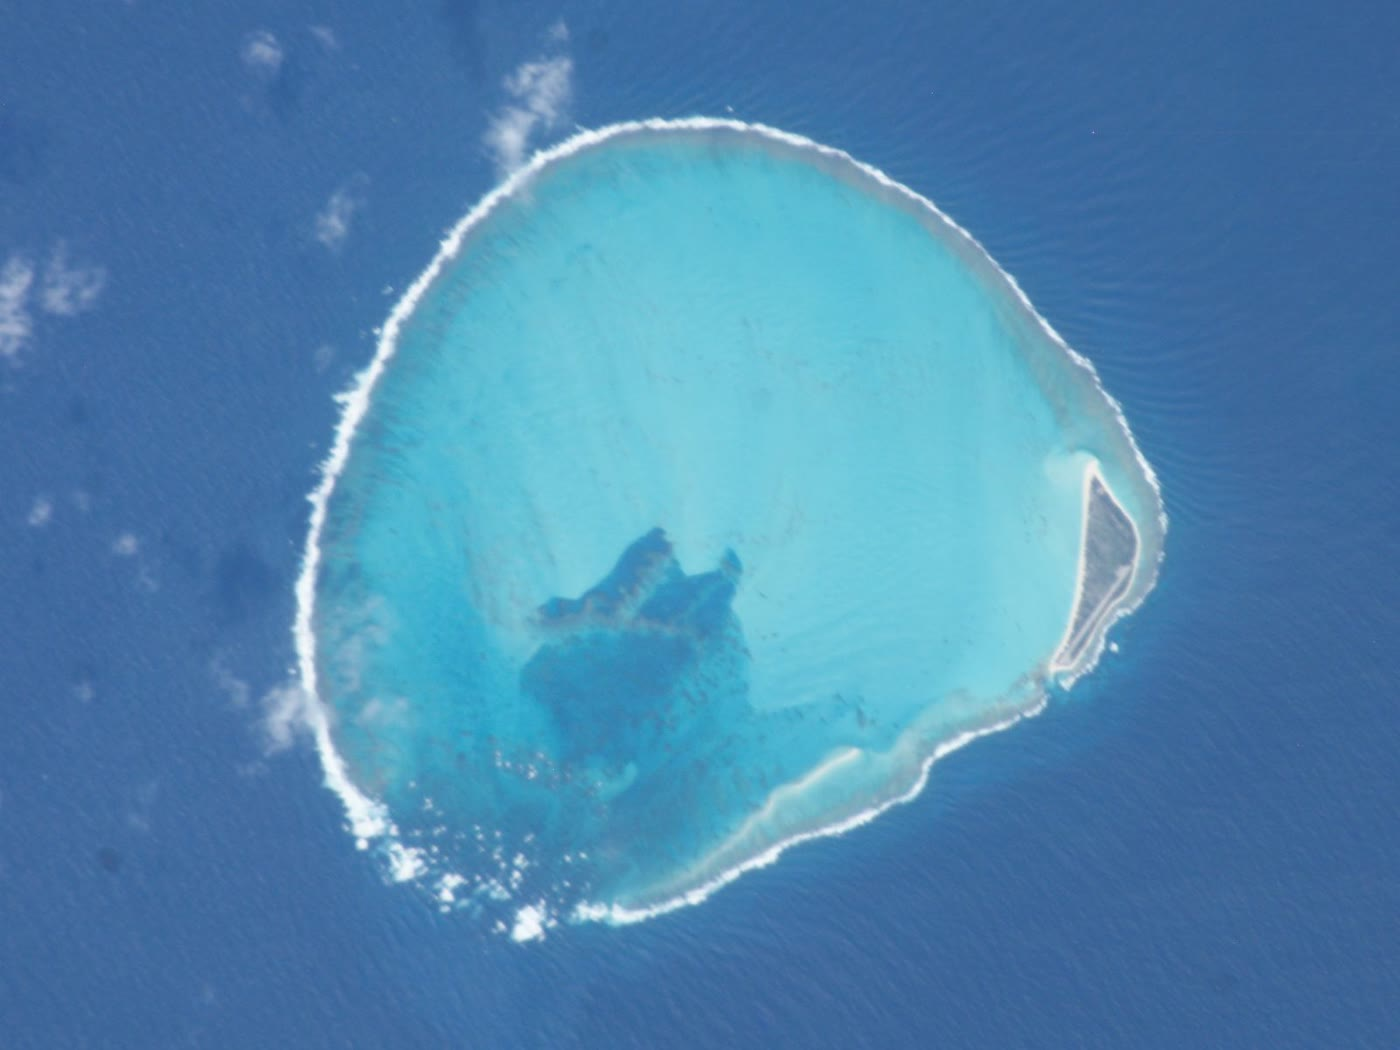
\includegraphics[width=0.52\linewidth]{images/book4/b2-17-kure-atoll.jpg}
\par\smallskip{\small حلقة كوري المرجانية، أشدّ الحلقات المرجانية شمالًا، صوّرها رائد فضاء من
محطة الفضاء الدولية في 22 فبراير 2004. وحلقة الشعاب، التي يبلغ عرضها نحو عشرة كيلومترات
على الأكثر، تحيط ببحيرة؛ والجزيرة الدائمة الوحيدة، الجزيرة الخضراء، تقع على الحافة (يمينًا). الصورة:
ناسا، ملك عام، عبر \mbox{\textdir TLT Wikimedia Commons}.}
\end{omfigure}
% ledger: pmnm:kure (6 miles = 9.7 km)

\section{الحتّ ومستوى البحر ونهاية جزيرة}\label{sec:b2:oceanic-islands:erosion}

بينما تغوص الجزيرة، تُبرى أيضًا. فالجزيرة العالية تعترض الرياح التجارية: فعلى
السفوح المواجهة للريح من براكين هاواي يهطل في بعض المواضع أكثر من \qty{9}{m} من المطر في السنة.
وتحفر الجداول أخاديد عميقة في أقلّ من مليون سنة، كما في كوهالا، في جزيرة هاواي.
وبعض الجروف الكبيرة التي عُدّت يومًا من عمل الحتّ وحده، مثل الجروف البحرية لشمال
مولوكاي، تُقرأ اليوم على أنها جدران رؤوس انزلاقات عملاقة، تراجعت منذ ذلك الحين. وتهاجم الأمواج الساحل
وتسوّي مصطبة نحت الأمواج عند مستوى البحر حوله. ويزيل الحتّ والغوص معًا كل أثر
للصخر البركاني فوق البحر في نحو \qty{15}{Myr}. وقمم غاردنر، وهي من ذلك العمر تقريبًا،
أقدم جزيرة في السلسلة لا يزال فيها صخر بركاني قائمًا فوق الماء. ووراءها نحو
الشمال الغربي لا توجد إلا جزر رملية وحلقات مرجانية وبراكين غارقة.
% ledger: cs14:erosion, cs14:erase

لا يثبت مستوى البحر بينما يجري هذا. ففي الذروة الجليدية الأخيرة كان أخفض من اليوم بنحو
\qty{120}{m}. وكان ساحل الجزيرة حينئذ أخفض على أجنحتها، والشعاب
التي تحفّها اليوم كانت أرضًا يابسة. ولمّا ذاب الجليد، ارتفع البحر بمعدّل \qty{12}{m}
كل ألف سنة على امتداد الانحسار الجليدي الرئيسي، من 16.5 إلى \qty{8.2}{ka}. وفي أثناء نبضة المياه
الذائبة \babelsublr{1A} ارتفع بما لا يقلّ عن \qty{40}{mm} في السنة. والشعاب على بركان يغوص يجب أن تتبع
الارتفاعين كليهما. وقبالة الساحل الشمالي الغربي لجزيرة هاواي، تشكّل ست شعاب غارقة على الأقلّ
درجًا على الجناح، أقدمها أعمقها. وقد نمت كلّ منها عند الشاطئ، ثم تخلّفت في أثناء ارتفاع
للبحر، وحملها إلى الأسفل تحميلُ الجزيرة الفتيّة. فإذا غاص بركان أكثر
من نحو \qty{125}{m}، أي مدى مستوى البحر الجليدي، فلن يعود صاعدًا إلى الأمواج.
% ledger: usgs:lgm (Book 1), lambeck14:lgm (Book 2), cs14:erase, cs14:subsidence

ويمكن للقوس أن يعمل في الاتجاه المعاكس. فأواهو تقع على الانتفاخ الذي رفعه حمل الجزر الأحدث،
وقد ارتفعت قليلًا: فشعاب آخر فترة بين جليدية، التي يتراوح عمرها من 133 إلى \qty{115}{ka}، تتكشّف حول
الجزيرة كلّها، وشعاب عمرها نحو \qty{334}{ka} تقف اليوم على ارتفاع \qty{21}{m} فوق مستوى البحر.
فنهاية \omterm{def:b2:oceanic-islands:stages}{الجزيرة المحيطية} مكتوبة إذن في صخورها وشعابها. فالحمم تبنيها، والانزلاقات
والمطر تهدمها، والأمواج تسوّيها، والصفيحة تحملها إلى الأسفل، والشعاب تحافظ على مكانها عند
السطح حتى يُغرقها هي أيضًا الماء البارد وارتفاع البحر.
% ledger: cs14:arch

\section*{التمارين}\label{sec:b2:oceanic-islands:exercises}

معطيات التمارين، ما لم يُذكر غير ذلك: قانون العمق--العمر $d = \qty{2500}{m} + C\sqrt t$ مع
$C = \qty{350}{m.Myr^{-1/2}}$ من أجل $0 \le t \le \qty{70}{Myr}$، و$d = \qty{6400}{m} -
\qty{3200}{m}\,e^{-t/62.8}$ بعد \qty{20}{Myr}؛ و$1~\text{قدم} = \qty{0.3048}{m}$، و$1~\text{قامة}
= \qty{1.8288}{m}$، و$1~\text{ميل} = \qty{1.609}{km}$؛ ونموّ الشعاب حتى \qty{4.2}{mm.yr^{-1}}.

\begin{exercise}[$\star$]\label{exo:b2:oceanic-islands:1}
سمِّ مرحلة كلّ بركان: (أ) جبل بحري قمّته تحت سطح البحر بمقدار \qty{975}{m}، يُخرج
حممًا قلوية؛ (ب) بركان فوق البقعة الساخنة، يُخرج حممًا ثولييتية بمعدّل عالٍ؛ (ج) بركان
خامد آخر مسيلاته، الأكثر قلوية من معظم الجزيرة، تغطّي الدرع؛ (د) جزيرة
تنفتح فيها، بعد صمت دام \qty{2}{Myr}، بضع فوّهات قلوية صغيرة؛ (ه) حلقة من الشعاب
حول بحيرة لا يُرى فيها أي صخر بركاني.
\end{exercise}

\begin{exercise}[$\star$]\label{exo:b2:oceanic-islands:2}
يُبنى بركان على صفيحة عمرها \qty{9}{Myr}. (أ) ما عمق قاع البحر من حوله؟ (ب) كم
سيكون قد غاص حين يصير عمر الصفيحة \qty{25}{Myr}؟ (ج) بأيّ معدّل يغوص حينئذ؟
\end{exercise}

\begin{exercise}[$\star$]\label{exo:b2:oceanic-islands:3}
تكوّن سبعة عشر انزلاقًا كبيرًا في آخر \qty{5}{Myr} حول جزر هاواي الرئيسية،
وسبعون على امتداد ظهرة هاواي في \qty{30}{Myr}. (أ) أوجد متوسط الفترة بين انزلاقين في
كل حالة. (ب) لماذا لا تكون الفترتان إلا حدّين أعليين للفترة الحقيقية؟
\end{exercise}

\begin{exercise}[$\star$]\label{exo:b2:oceanic-islands:4}
في إنيويتاك، صودف البازلت عند 4158 قدمًا في بئر والأساس الصلب عند 4610 أقدام في
الأخرى؛ ومرجانيات الشعاب عند قاعدة الحجر الجيري لا تعيش أعمق من 150 قدمًا. (أ) حوّل
الأعماق الثلاثة إلى أمتار. (ب) بمقدار كم على الأقلّ غاصت قمّة البركان تحت جزيرة باري
منذ نمت عليها أولى الشعاب؟ (ج) قاعدة الحجر الجيري إيوسينية، فعمرها لا يقلّ عن
\qty{33.9}{Myr}. ما أكبر معدّل متوسط ممكن للغوص؟
\end{exercise}

\begin{exercise}[$\star\star$]\label{exo:b2:oceanic-islands:5}
(أ) أوجد معدّل الغوص الحراري، بوحدة \unit{m} لكل \unit{Myr} وبوحدة \unit{mm.yr^{-1}}، لجزر
على صفائح أعمارها 4 و25 و\qty{49}{Myr}. (ب) كم مرة أسرع من أسرعها
يمكن أن تنمو شعاب منتجة؟ (ج) وكم مرة أسرع تكون مرحلة التحميل قبالة جزيرة
هاواي، \qty{2.6}{m} لكل ألف سنة؟
\end{exercise}

\begin{exercise}[$\star\star$]\label{exo:b2:oceanic-islands:6}
(أ) بالقانون الأسّي، أوجد معدّل الغوص على صفيحة عمرها \qty{100}{Myr}، بوحدة \unit{m}
لكل ألف سنة، وقارنه بمعدّل \qty{0.01}{m} لكل ألف سنة المقيس على امتداد
ظهرة هاواي. (ب) عند أيّ عمر للصفيحة يكون المعدّل \qty{10}{m.Myr^{-1}} بالضبط؟ (ج) تحقّق من أن
القانونين يعطيان العمق نفسه تقريبًا لصفيحة عمرها \qty{25}{Myr}.
\end{exercise}

\begin{exercise}[$\star\star$]\label{exo:b2:oceanic-islands:7}
تغرق شعاب هاواي بعد نحو \qty{33}{Myr} من ولادة بركانها، ويتنقّل النشاط البركاني
على امتداد السلسلة بسرعة \qty{8.6}{cm.yr^{-1}}. (أ) على أيّ بعد من البقعة الساخنة تقع جزيرة حين
تغرق شعابها؟ (ب) ميدواي حلقة مرجانية عمرها \qty{27.7}{Myr}: أيتّسق ذلك مع أنها لا تزال تحمل
شعابًا حيّة؟ (ج) تقع كوري على بعد 55 ميلًا وراء ميدواي. قدّر عمرها، وقل هل هي قريبة
من \omterm{def:b2:oceanic-islands:darwin-point}{نقطة داروين}.
\end{exercise}

\begin{exercise}[$\star\star$]\label{exo:b2:oceanic-islands:8}
في \omterm{def:b2:oceanic-islands:collapse}{الانهيار الركامي} لنووانو، جبل توسكالوسا البحري كتلة طولها نحو \qty{30}{km}،
وعرضها \qty{17}{km} وارتفاعها لا يقلّ عن \qty{2}{km}. (أ) ما الحجم الذي يسعه صندوق بهذه الأبعاد؟
وهرم له القاعدة نفسها والارتفاع نفسه؟ (ب) قارن بحجم
كيلاويا، \qty{10000}{km^3}. (ج) يغطّي الانهيار \qty{23000}{km^2}. فلو كان سمكه في المتوسط
\qty{100}{m} (افتراض: فسمكه بعيدًا عن أواهو غير معروف جيدًا)، فكم يكون
حجمه؟
\end{exercise}

\begin{exercise}[$\star\star$]\label{exo:b2:oceanic-islands:9}
قبالة جزيرة هاواي يغوص الجناح بمقدار \qty{2.6}{m} لكل ألف سنة تحت حمل
البركان. (أ) كم من الوقت يلزم لإغراق خطّ شاطئ بمقدار \qty{1}{km}؟ (ب) شعاب تنمو بمعدّل
\qty{4.2}{mm.yr^{-1}} تقع على هذا الجناح. هل تجاري حين يكون مستوى البحر ثابتًا؟ (ج) في أثناء
الانحسار الجليدي الرئيسي، من 16.5 إلى \qty{8.2}{ka}، ارتفع البحر بمعدّل \qty{12}{mm.yr^{-1}} في المتوسط. ما
عمق قمّة الشعاب في النهاية، إذا بدأت عند السطح؟ (د) السؤال نفسه، لشعاب على
بركان قديم لم يعد يغوص.
\end{exercise}

\begin{exercise}[$\star\star\star$]\label{exo:b2:oceanic-islands:10}
(أ) بيّن أنه، على فترة ثابتة $\Delta$، يجعل قانون الجذر الجزيرة تغوص أقلّ كلّما كانت صفيحتها
أقدم. (ب) احسب الغوص خلال \qty{20}{Myr} لجزيرة وُلدت عند الظهرة ولأخرى وُلدت
على صفيحة عمرها \qty{50}{Myr}. (ج) الصفيحة تحت الظهرة حارّة جدًا، وقانون الجذر يعطي
معدّلًا لانهائيًا عند $t = 0$. هل هذه مشكلة للغوص على فترة منتهية؟ علّل.
\end{exercise}

\begin{exercise}[$\star\star\star$]\label{exo:b2:oceanic-islands:11}
تغوص حلقة مرجانية بمعدّل \qty{30}{m.Myr^{-1}}، ويتأرجح مستوى البحر بنحو \qty{120}{m} مع العصور
الجليدية، في دورات طولها نحو \qty{100}{kyr}. (أ) كم تغوص \omterm{def:b2:oceanic-islands:reefs}{الحلقة المرجانية} في دورة واحدة؟ (ب) عند
انخفاض جليدي، كم ترتفع قمّة \omterm{def:b2:oceanic-islands:reefs}{الحلقة المرجانية} فوق البحر؟ وماذا يحدث لصخر
الشعاب حينئذ؟ (ج) كم دورة يلزم لتغوص \omterm{def:b2:oceanic-islands:reefs}{الحلقة المرجانية} بكامل \qty{120}{m}؟
(د) فسّر النطاقات المغسولة الموجودة في آبار إنيويتاك، ولماذا
تظلّ \cref{prop:b2:oceanic-islands:cap} تعطي سمك الغطاء على المدى الطويل.
\end{exercise}

\begin{exercise}[$\star\star\star$]\label{exo:b2:oceanic-islands:12}
تغرق حلقة مرجانية حين يكون عمر صفيحتها \qty{50}{Myr}: فتتخلّف شعابها وتنتهي قمّتها عند
حدّ نموّ أعمق الطحالب المرجانية، \qty{150}{m} تحت سطح البحر. (أ) بالقانون
الأسّي، كم تغوص بعد ذلك قبل أن يصير عمر الصفيحة \qty{120}{Myr}؟ (ب) ما عمق قمّة
\omterm{def:b2:oceanic-islands:seamount}{الغيوت} حينئذ؟ (ج) غيوت بجوار إنيويتاك قمّته عند 700 قامة. حوّل، وقارن.
(د) اذكر سببين يجعلان غيوتًا حقيقيًا أعمق أو أضحل من هذا التقدير.
\end{exercise}

\begin{problem}[{مسألة نهاية الأسبوع --- من بركان إلى حلقة مرجانية}]\label{pb:b2:oceanic-islands:1}
تولد جزيرة بترل المختلقة فوق بقعة ساخنة على صفيحة عمرها \qty{10}{Myr}. وبركانها
مخروط نصف قطر قاعدته \qty{50}{km}. وحين ينتهي نموّه، تعلو قمّته \qty{1000}{m} فوق
مستوى البحر. ويختفي آخر صخر بركاني فيها تحت مستوى البحر بعد \qty{12}{Myr}. ثم تُبقي
شعاب قمّتها عند مستوى البحر حتى يصير عمر الصفيحة \qty{70}{Myr}، حين تعبر \omterm{def:b2:oceanic-islands:reefs}{الحلقة المرجانية}
\omterm{def:b2:oceanic-islands:darwin-point}{نقطة داروين}. استعمل قانون العمق--العمر في التمارين (قانون الجذر حتى \qty{70}{Myr}، والقانون
الأسّي بعده)، ونموًّا للشعاب قدره \qty{4.2}{mm.yr^{-1}}، ومعطيات الفصل.
ويُعدّ مستوى البحر ثابتًا، إلا في الأسئلة من 8 إلى 10. دوّر الأعماق إلى المتر.

\noindent\textbf{الجزء الأول --- النموّ.}
\begin{enumerate}
  \item ما عمق قاع البحر حيث تولد بترل؟
  \item ما ارتفاع البركان فوق ذلك القاع حين ينتهي نموّه، مع إهمال
        غوص القاع تحت الحمل؟
  \item أوجد حجم المخروط.
  \item إذا ثار \qty{85}{\percent} منه في أثناء مرحلة درع دامت \qty{1}{Myr}، فما كان
        المعدّل المتوسط للثوران؟ قارن بإمداد كيلاويا اليوم، نحو
        \qty{0.1}{km^3} في السنة.
  \item كم بترل يلزم لتكوين ماونا لوا واحد، بحجم \qty{95600}{km^3}؟
  \item أيّ الحمم، الثولييتية أم القلوية، تكوّن معظم المخروط؟ وأيّها تغطّيه؟
\end{enumerate}

\noindent\textbf{الجزء الثاني --- التحميل والشعاب الغارقة.}
\begin{enumerate}[resume]
  \item في أثناء نموّها، يُغوِّص الحمل الجزيرة الفتيّة بمقدار \qty{1}{km} في \qty{1}{Myr}. ما
        المعدّل المتوسط، وكيف يقارن بمعدّل \qty{2.6}{m} لكل ألف سنة المقيس
        قبالة جزيرة هاواي؟
  \item تنمو شعاب على الشاطئ في أثناء هذه المرحلة، ومستوى البحر ثابت. هل تجاري،
        وبأيّ هامش؟
  \item ثم يرتفع مستوى البحر بمعدّل \qty{12}{mm.yr^{-1}}. بكم تتخلّف الشعاب كل
        سنة؟
  \item كم من الوقت قبل أن تبلغ قمّتها \qty{150}{m}، أعمق حدّ للنموّ؟ وماذا يترك ذلك
        على جناح الجزيرة؟
\end{enumerate}

\noindent\textbf{الجزء الثالث --- الغوص والحتّ.}
\begin{enumerate}[resume]
  \item بكم تكون بترل قد غاصت حين يختفي آخر صخر بركاني فيها، وعمر الصفيحة
        حينئذ \qty{22}{Myr}؟
  \item كم أزال الحتّ من ارتفاع القمّة البالغ \qty{1000}{m}، وبأيّ معدّل متوسط؟
  \item بأيّ معدّل تغوص بترل حين ينتهي نموّها، وحين تختفي قمّتها؟
  \item ما عمق قاع البحر من حولها حينئذ؟
  \item قارن المدّة \qty{12}{Myr} التي استغرقتها بمدّة \qty{15}{Myr} لجزر هاواي. واذكر
        سببًا يجعل جزيرة هاواي العالية تدوم أطول.
  \item اذكر عمليّتين، غير المطر والأنهار، تزيلان الجزيرة فوق مستوى البحر.
  \item أيّ نوع من الشعاب يحيط ببترل قبيل اختفاء قمّتها؟
\end{enumerate}

\noindent\textbf{الجزء الرابع --- \omterm{def:b2:oceanic-islands:reefs}{الحلقة المرجانية} \omterm{def:b2:oceanic-islands:seamount}{والغيوت}.}
\begin{enumerate}[resume]
  \item ما سمك غطاء الشعاب حين يكون عمر الصفيحة \qty{70}{Myr}؟
  \item ما المعدّل المتوسط لنموّ الشعاب الذي تطلّبه ذلك؟ وكم مرة يصغر عن النموّ
        الذي كان يمكن للشعاب بلوغه؟
  \item قارن الغطاء بعمق البازلت تحت إنيويتاك.
  \item ما عمق قاع البحر حول \omterm{def:b2:oceanic-islands:reefs}{الحلقة المرجانية} حين تعبر \omterm{def:b2:oceanic-islands:darwin-point}{نقطة داروين}؟
  \item بالقانون الأسّي، كم تغوص \omterm{def:b2:oceanic-islands:reefs}{الحلقة المرجانية} الغارقة بعد ذلك قبل أن يصير عمر الصفيحة
        \qty{120}{Myr}؟
  \item إذا توقّفت قمّة الشعاب عند \qty{150}{m} حين غرقت، فما عمق قمّة
        \omterm{def:b2:oceanic-islands:seamount}{الغيوت} حينئذ؟
  \item خلاصة: ما سمك غطاء الشعاب لحلقة بترل المرجانية؟
\end{enumerate}
\end{problem}
